% 0609/scan
\chapter{Camera}
\label{sec:rigid}
In order to relate coordinates on the LCoS display with pixel
positions on the camera, we found it suffices to use a rigid
transform. The rigid transform between display and camera is defined
as:
\begin{align}
  \r^d&=s \textrm{R}_\phi \r^c + \vect t\\
  \textrm{R}_\theta&=\begin{pmatrix}
  \cos\phi & q\sin\phi \\
  -\sin\phi & q\cos\phi \\ 
  \end{pmatrix}
\end{align}
where $\r^d$ is a point on the display, $\r^c$ is a point on the
camera and $q$ can be either $+1$ or $-1$ dependent on if there is a
reflection.

\begin{figure}[!hbt]
  \centering
  \input{calib-align.eps_tex}
  \caption{Given $n>3$ camera images of a display showing one point it
    is possible to calculate the parameters of the rigid transform
    parameters scaling $s$, rotation angle $\phi$, translation vector
    $\vect t$.}
  \label{fig:calib-align}
\end{figure}



One can find the transform parameters scaling $s$, rotation angle
$\phi$, translation vector $\vect t$ by minimizing
\begin{align}
  \sum_i^n \abs{s \textrm{R}_\phi \r^c_i+\vect t -\r^d_i}^2
\end{align}
for all $n$ points on the display $\r^d_i$ and there corresponding
camera positions $\r^c_i$.  Each term of the sum can be expressed as
two scalar terms:
\begin{align*}
  \sum_i^n&
  \abs{s(\cos\phi r^c_{ix}+q\sin\phi r^c_{iy})+t_x-r^d_{ix}}^2\\
  &+
  \abs{s(-\sin\phi r^c_{ix}+q\cos\phi r^c_{iy})+t_y-r^d_{iy}}^2
\end{align*}

The following Maxima code will find the solution to the least squares
problem:
\begin{verbatim}
load(minpack)$
q:-1;
g(s,p,tx,ty):=[
s*( cos(p)*<cx>+q*sin(p)*<cy>)+tx-<dx>,
s*(-sin(p)*<cx>+q*cos(p)*<cy>)+ty-<dy>
...
]$
minpack_lsquares(
  g(s,p,x,y),
  [s,p,x,y],
  [0.88,-3.1,1200,-20]);
\end{verbatim}
We define the function \verb!g! to contain all the terms of the sum.
This can easily written by a program that constructs the lines
according to the given pattern, replacing \verb!<cx>!, \verb!<cy>!
with camera coordinates and \verb!<dx>!, \verb!<dy>! with display
coordinates.

The function \verb!minpack_lsquares! calls the subroutine \verb!lmder!
from the Fortran package \verb!minpack!.
{\small
\begin{verbatim}
c     subroutine lmder (http://www.netlib.org/minpack/lmder.f)
c
c     the purpose of lmder is to minimize the sum of the squares of
c     m nonlinear functions in n variables by a modification of
c     the levenberg-marquardt algorithm. the user must provide a
c     subroutine which calculates the functions and the jacobian.
c
c     the subroutine statement is
c
c       subroutine lmder(fcn,m,n,x,fvec,fjac,ldfjac,ftol,xtol,gtol,
c                        maxfev,diag,mode,factor,nprint,info,nfev,
c                        njev,ipvt,qtf,wa1,wa2,wa3,wa4)
\end{verbatim}}

An advantage of using Maxima is, that it conveniently calculates
the symbolic jacobian for the problem.

The following Common Lisp code shows how the result of the
optimization can be used to initialize the OpenGL modelview matrix to
transform objects in its buffer, so that they will appear at the given
positions on the camera.

{\small\begin{verbatim}
(defun load-cam-to-lcos-matrix (&optional (x 0s0) (y 0s0))
  (let* ((s 0.828333873909549)
         (sx  s)
         (sy  (- s))
         (phi -3.101722728951688)
         (sp (sin phi))
         (cp (cos phi))
         (tx 608.4330743004457)
         (ty 168.9188383630887)
         (a (make-array
             (list 4 4) :element-type 'single-float
             :initial-contents
             (list (list (* sx cp)    (* sy sp)  .0  (+ x tx))
                   (list (* -1 sx sp) (* sy cp)  .0  (+ y ty))
                   (list .0     .0   1.0  .0)
                   (list .0     .0    .0 1.0)))))
    (gl:load-transpose-matrix (sb-ext:array-storage-vector a))))    
\end{verbatim}}
  
  Alternatively, here is the equivalent code in C:

{\small\begin{verbatim}
float m[4*4]; // OpenGL Modelview Matrix
float s=-.8749328910202312,
      sx=s,sy=-s,phi=-.8052030670943575,
      cp=cos(phi),sp=sin(phi),
      tx=1456.71806436377,
      ty=910.4787738693659;
  m[0]=sx*cp;
  m[1]=-1*sx*sp;
  m[2]=0;
  m[3]=0;
  
  m[4]=sy*sp;
  m[5]=sy*cp;
  m[6]=0.;
  m[7]=0.;

  m[8]=0;
  m[9]=0;
  m[10]=1;
  m[11]=0;
  
  m[12]=tx;
  m[13]=ty;
  m[14]=0;
  m[15]=1;
glMatrixMode(GL_MODELVIEW);
glLoadMatrixf(m);
\end{verbatim}}

For the calibration a fluorescent plane like in

\begin{figure}[!hbt]
  \centering
  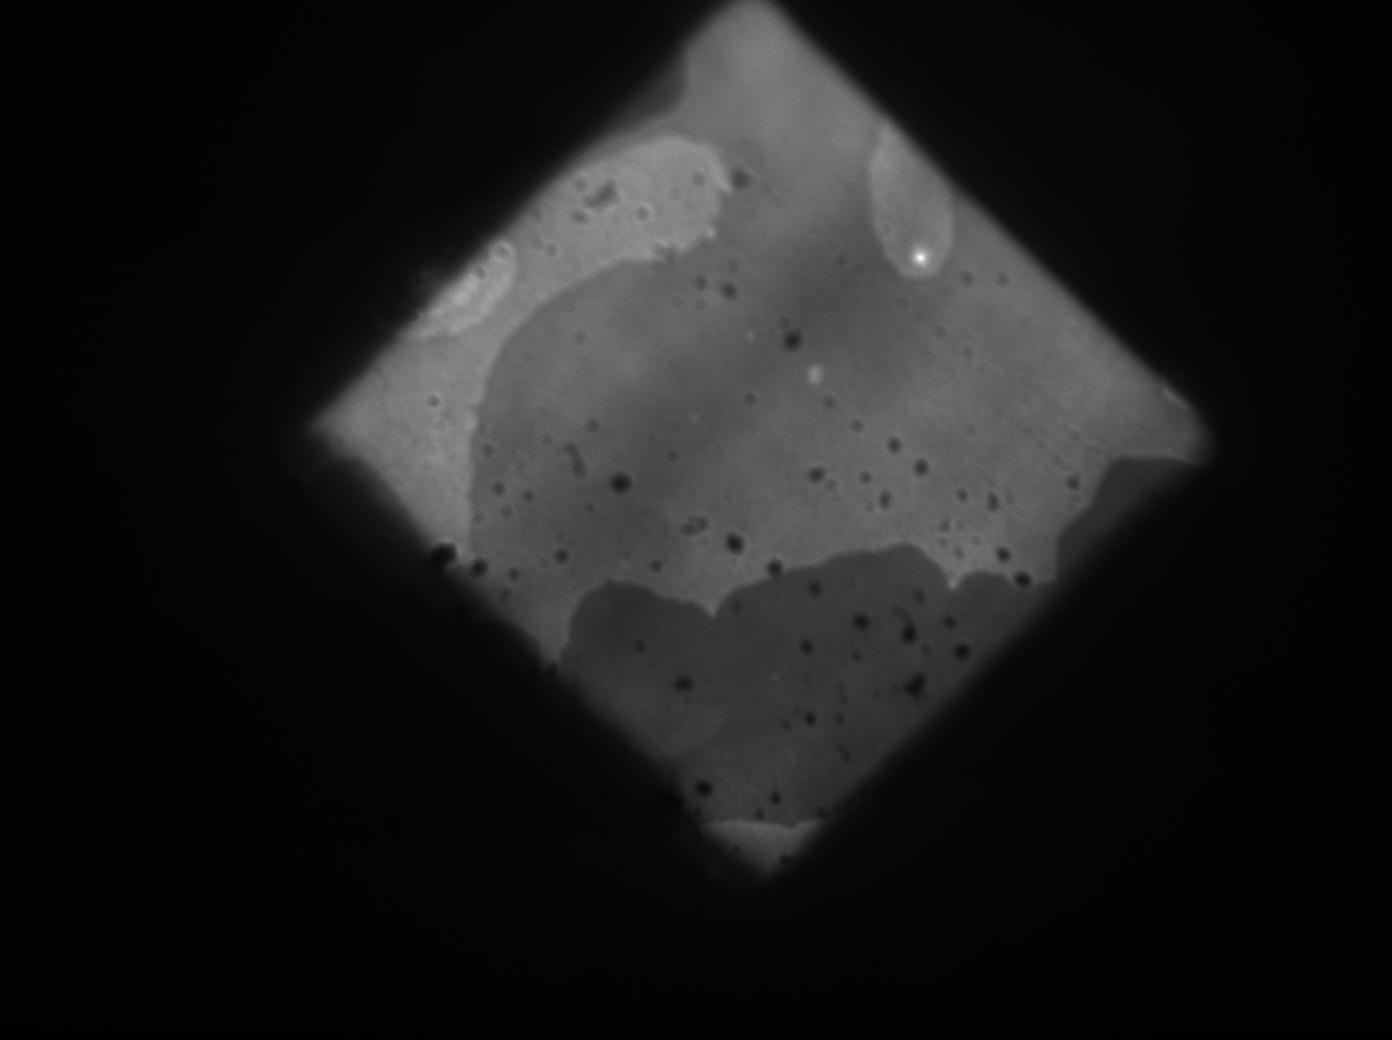
\includegraphics[width=7cm]{o102}
  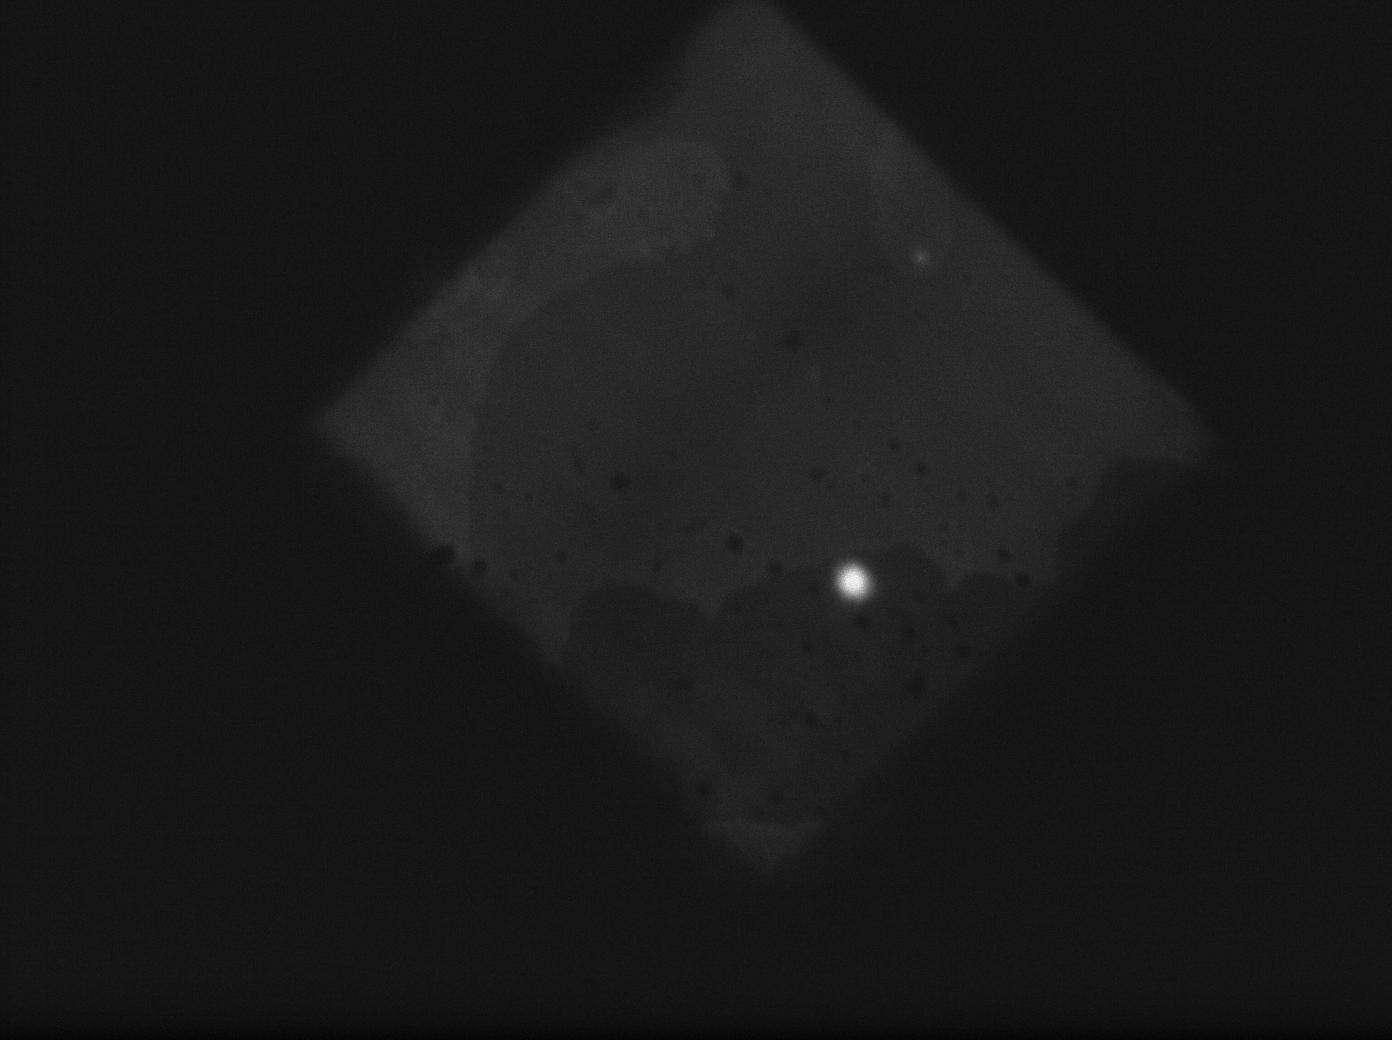
\includegraphics[width=7cm]{o035}
  \caption{{\bf left:} Uniformly illuminated flourescent plane (mono
    and double layer of yellow beads with \unit[110]{nm} diameter,
    excited with \unit[473]{nm} laser in a 63x/1.47 objective). {\bf
      right:} Image with the the LCoS displaying a disk with 24 pixels
    diameter (corresponding to $\unit[2.4]{\mu m}$ in the sample)
    centered at LCoS position $(550,750)$. For this image all mirrors
    on the MMA are undeflected and its Fourier apertures $B_0$ and
    $B_1$ completely open.}
  \label{fig:rigid-pics}
\end{figure}

% i believe the TL_ill is set to r_MMA=3.84mm in BFP 
% f_TLill = 352 mm
% mag_real = mag / f_zeiss * f_TLill 
% pixel-pitch-lcos / mag_real
% one pixel is: 13.62 / 63 * 164.5 / 352 = 101nm

\begin{figure}[!hbt]
  \centering
  \includegraphics[width=12cm]{screen_rigid-transform}
  \caption{dfaxs}
  \label{fig:screen_rigid-transform}
\end{figure}


{\small
\begin{verbatim}
%% load the files
cd /mnt/scan
a = newim(1392,1040,103);
tic % 51s
for i=0:102
    % the values are negative, maybe fits can't be read correctly
    a(:,:,i) = 2^15 + readim(sprintf('o%03d.fits',i));
end
toc

% 0 .. 99 spot images
% only from 10.99 usable because the first are on border
% 100 small disk in center
% 101 should be different disk but looks weird
% 102 uniform illumination

%% bright image is at 102
diphist(a(:,:,102),[min(a),max(a)])

%% minimum at -3.2e4 (or 800)
bright = squeeze(a(:,:,102));
mask = gaussf(bright,8) > 800;

%% i forgot to capture a dark image, but from the histogram of the
%% first spot image i estimate the background to be 510
diphist(a(:,:,0),[min(a),max(a)])   
%%
bg = 510;
%%
% (a - bg) / repmat(bright,[1 1 103]) * repmat(mask,[1 1 103])

posmax = newim(100,2);
for i = 10:99
    % correct for sample non-uniformity with homogene image (102)
    corr = (squeeze(a(:,:,i)) - bg) / bright * mask;
    % find coordinates of maximum
    [coords,vals]=findmaxima(gaussf(corr,32));
    [valss,valsind] = sort(vals);
    tmp = coords(valsind,:);
    posmax(i,:) = tmp(end,:);
end

%% store the positions as ascii text
q = double(posmax)';
save /dev/shm/o.mat q -ASCII  -DOUBLE

%% create maxima input for optimization
c = double(posmax)'; % camera

cmd = '';
for i=10:99
    dx = num2str(400+50*mod(i,10));
    dy = num2str(500+50*floor(i./10));
    cx = num2str(c(i+1,1));
    cy = num2str(c(i+1,2));
    cmd=[cmd ' s*( cos(p)*' cx '+q*sin(p)*' cy ')+tx-' dx ',s*(-sin(p)*' ...
         cx '+q*cos(p)*' cy ')+ty-' dy ','];
end

cmd(:,end) = []; % delete last comma

% load the fitting package and start defining the merit function g
pre = 'load(minpack)$ q:-1; g(s,p,tx,ty):=[';
% now put cmd between
% call the fitting function and store the parameters into /dev/shm/max.out
cod = [']$ fit:minpack_lsquares(g(s,p,x,y),[s,p,x,y],[.88,-1.3,1200,-20]); write_data(fit[1],"/home/martin/max.out");']


%% write maxima commands into file
fid = fopen('/dev/shm/fit.max','w');
fwrite(fid,[pre cmd cod]);
fclose(fid);
[max_status,max_result]=system('maxima -b /dev/shm/fit.max');

%% load rigid transformation parameters from the file into matlab
params = load('/home/martin/max.out')';
scale = params(1);
phi = params(2);
tx = params(3);
ty = params(4);

mirr = -1;
R = [cos(phi),mirr*sin(phi);
     -sin(phi),mirr*cos(phi)];
T = [tx ty]';

%% plot the two grids on top of each other

% transform camera coordinates into display coordinates
mapped = zeros(100,2);
for i=11:100
    mapped(i,:) = (scale*R*q(i,:)'+T)';
end

% calculate display points
dpos = zeros(100,2);
for i=0:99
    dpos(i+1,1) = 400+50*mod(i,10);
    dpos(i+1,2) = 500+50*floor(i./10);
end


hold off;
plot(dpos(:,1),dpos(:,2),'.');
hold on;
plot(mapped(11:end,1),mapped(11:end,2),'r+');
% plot([0 1280],[0 1024],'+'); % show full display
\end{verbatim}}
